% !TEX root = ../TechProject.tex

\graphicspath{{Chapter5/}}


\chapter{Experiment}


As explained in the hypothesis. a music recommendation system that uses \textit{MixesDB} as a dataset was made. An experiment was ran to see if it garners appropriate results, and will help answer the following question:
\\
\\
\textit{Is the proposed method a suitable solution to automate recommendations of songs suitable for adding to a given DJ set?}.
\\

To evaluate the quality of a recommendation system, R-Precision is often used as a performance metric. 
\\

\section{R-Precision}

\begin{equation}
	R-Precision = \frac{|G\cap R_{1:|G|}|}{|G|}
\end{equation}
\\\\
R-precision is the amount of found tracks that were originally in the mix divided by the number of known missing tracks. This is shown in the equation in 6.1 allowing $G$ to be the set of missing songs, and $R$ to be the set of recommanded songs.

R-Precision was used in the 2018 \textit{Recsys} Convention idea for testing submissions for the million playlist challenge dataset from \textit{Spotify} \citep{aicrowd_aicrowd_2023}. At this convention, competing teams built recommendation system trained with the \textit{Spotify} dataset. To tests its quality, a challenge dataset, which contained many modified playlists, was used to test the models.

It is important to note the considerable difference in the number of DJ sets/playlists between the \textit{MixesDB} and the \textit{Spotify} dataset. The \textit{MixesDB} dataset contains over 9800 DJ sets, while the Spotify dataset contains 1,000,000 playlists. The differences between playlists and DJ sets is worth mentioning as well. A playlist being a collection of songs, regardless of cohesion or song count, while a DJ set is typically a seamless mix of songs that can vary in length from 8 hours to no less than 20 minutes.
\\
\\
The top 10 scoring models from the convention have R-Precision values ranging from 0.21 to 0.22. Given the differences in dataset size and task, aiming for an average R-Precision value of 0.171, slightly lower than the top-performing models, would be appropriate. Achieving this value would rank the model within the top 30 models trained by members of the public on the given \textit{Spotify} dataset \citep{aicrowd_aicrowd_2023}. This approach allows for a fair comparison between the different systems and considers the unique characteristics of the dataset and task at hand. 

As the dataset utilized with the proposed model was obtained from \textit{MixesDB}, a customized approach for the preparation of the evaluation set was conducted.

\section{Preparing Evaluation Set}
During the evaluation phase of the million playlist challenge, the quality of a given applications trained on this dataset was assessed through a range of methods that involved analysing both missing and recommended songs. In order to effectively compare different applications, it was essential to create a standardised evaluation set that incorporated aspects of the Spotify data set, to show if a submitted applications could recommend songs that were featured in the original playlist.

\begin{figure}[H]
	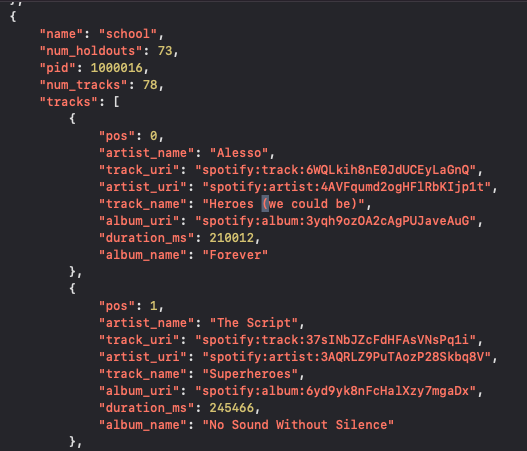
\includegraphics[scale=0.5]{images/spotify_challenge_set}
	\centering
	\caption{Screenshot of spotify challenge set. \citep{aicrowd_aicrowd_2023}} 
\end{figure}

The Spotify challenge set consisted of 10,000 playlists with varying numbers of input songs, ranging from 0 to 100 tracks. For each of these playlists, Spotify requested 500 track recommendations from the participating teams \citep{aicrowd_aicrowd_2023}. However, due to the smaller scale of the dataset and difference between playlists and DJ sets under consideration, various aspects of the  challenge set used on the proposed model had to be downscaled. For instance, the range of input songs was considerably narrower, as DJ sets typically have a minimum length of 10 tracks, compared to playlists that can have varying lengths.
\\
\\
To ensure all songs in the evaluation set could be found, each song had to have a total play count of at least 5. This means each song had to be played a total of 5 times by other DJ's within the training set. This value was chosen to ensure that each song in the set would likely be found in the training set. Furthermore, the input and missing songs were split in the following way, with 20\% of the songs allocated as missing songs, and the remaining 80\% as input songs. This was done to ensure enough songs were inputted. The output value for the application was also changed from 10 to 100 to better match the output for the evaluation given for the \textit{Spotify} dataset.

The making of the evaluation set was coded in \textit{Python} using the \textit{pandas} library and \textit{pytest} was used for unit-testing.
\\
\\
\begin{figure}[H]
	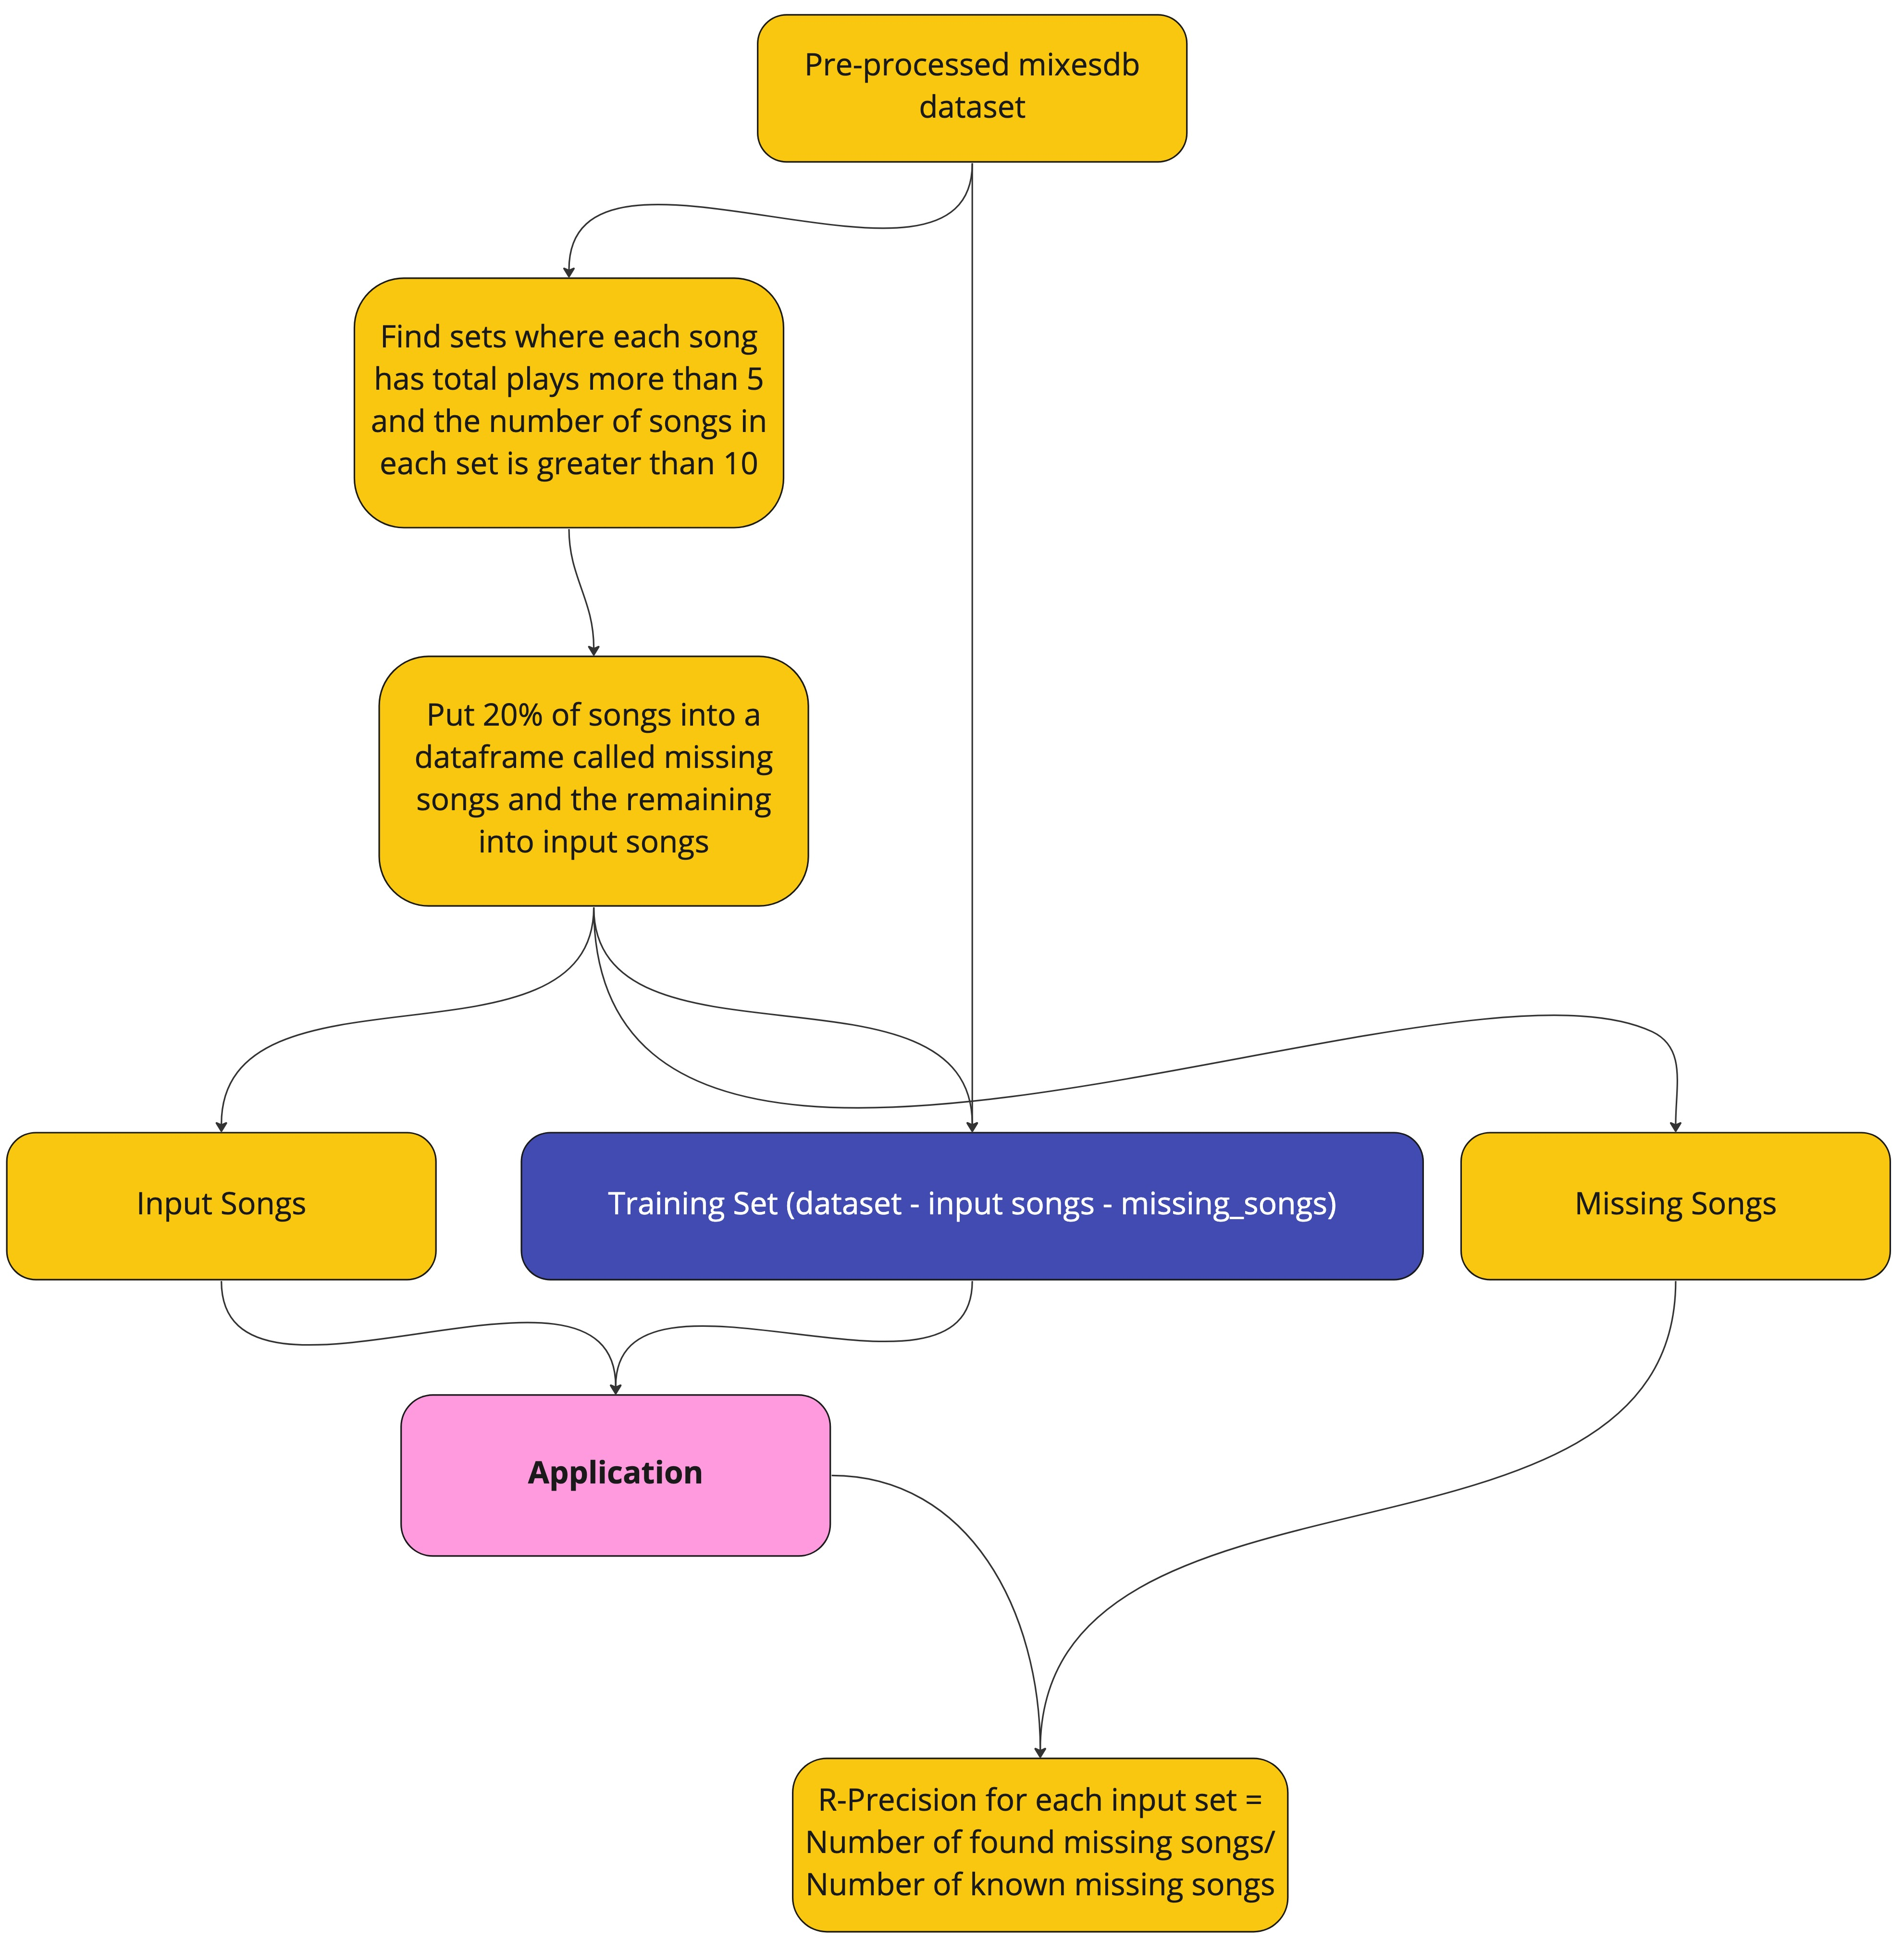
\includegraphics[scale=0.1]{images/evaluation_set_app_flow}
	\centering
	\caption{Application flow of the creation of the evaluation set} 
\end{figure}

\section{Experiment Variables}

As mentioned in chapter 5, the proposed application utilises the alternating least squares algorithm to generate an initial set of suggestions. This algorithm is based on matrix factorization, where the latent factors are derived from the training dataset to identify similar songs. The selection of an appropriate value for latent factors is crucial in ensuring the optimal performance of the algorithm. A low latent factor value may yield random results , while a value that is too high may lead to over-fitting \citep{zhou_large-scale_2008}. To identify the ideal value for latent factors, it is necessary to conduct an  investigation where the latent factors will be the independent variable, and the average R-precision value will be the dependent variable. 

Once the best R-precision value is obtained, an examination on how changes to the size of the input DJ sets, impact the R-Precision value. From there, the R-precision value is then compared to the highest performing recommendation systems that use the Spotify Dataset, to see if the DJ set focused recommender can compare to industry standard models.

The experiment was ran on a 16GB 2020 MacBookPro.

\section{Summary}
An overview of the \textit{Spotify} challenge set was given. The changes that had to be made to create a challenge set out of the \textit{MixesDB} dataset was explained. It was  shown how the evaluation set was made. 

The description on the test plan was shown. The initial independent variable was latent factors, and then the input DJ set size. The experiment will be concluded with a comparision in R-Precision scores with top performing models trained on the \textit{Spotify} dataset.

